% Created by tikzDevice version 0.10.1 on 2017-11-27 12:50:20
% !TEX encoding = UTF-8 Unicode
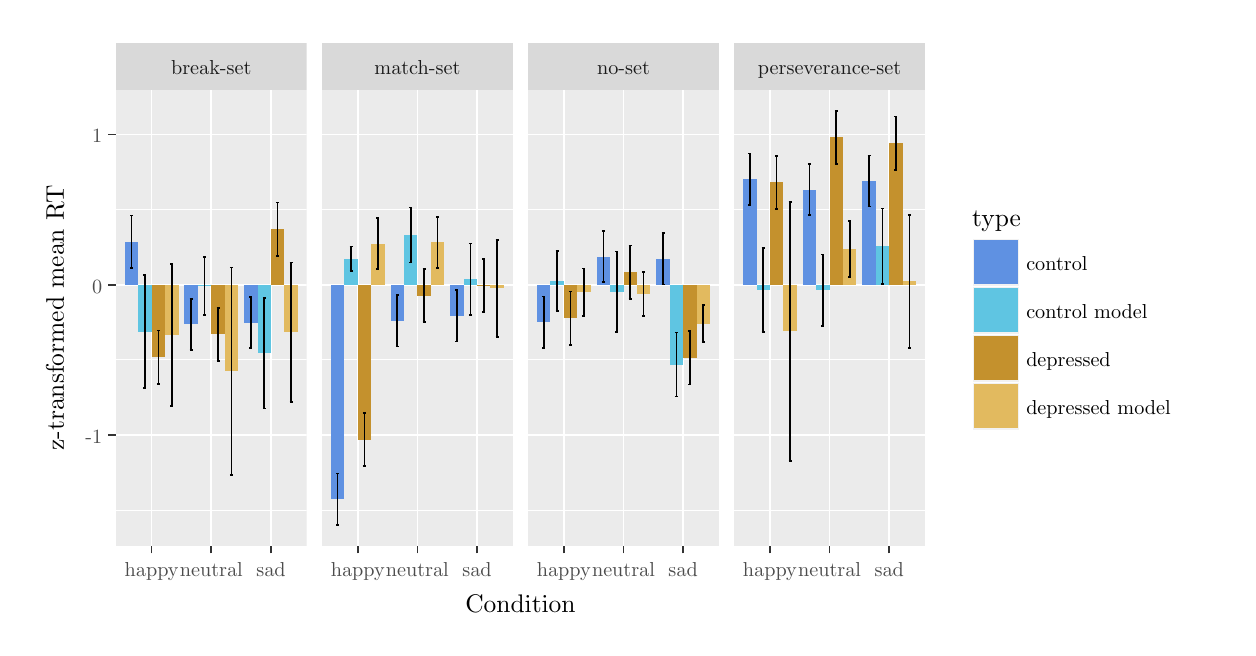
\begin{tikzpicture}[x=1pt,y=1pt]
\definecolor{fillColor}{RGB}{255,255,255}
\path[use as bounding box,fill=fillColor,fill opacity=0.00] (0,0) rectangle (433.62,216.81);
\begin{scope}
\path[clip] (  0.00,  0.00) rectangle (433.62,216.81);
\definecolor{drawColor}{RGB}{255,255,255}
\definecolor{fillColor}{RGB}{255,255,255}

\path[draw=drawColor,line width= 0.6pt,line join=round,line cap=round,fill=fillColor] (  0.00,  0.00) rectangle (433.62,216.81);
\end{scope}
\begin{scope}
\path[clip] ( 31.87, 29.59) rectangle (100.84,194.25);
\definecolor{fillColor}{gray}{0.92}

\path[fill=fillColor] ( 31.87, 29.59) rectangle (100.84,194.25);
\definecolor{drawColor}{RGB}{255,255,255}

\path[draw=drawColor,line width= 0.3pt,line join=round] ( 31.87, 42.48) --
	(100.84, 42.48);

\path[draw=drawColor,line width= 0.3pt,line join=round] ( 31.87, 96.76) --
	(100.84, 96.76);

\path[draw=drawColor,line width= 0.3pt,line join=round] ( 31.87,151.03) --
	(100.84,151.03);

\path[draw=drawColor,line width= 0.6pt,line join=round] ( 31.87, 69.62) --
	(100.84, 69.62);

\path[draw=drawColor,line width= 0.6pt,line join=round] ( 31.87,123.90) --
	(100.84,123.90);

\path[draw=drawColor,line width= 0.6pt,line join=round] ( 31.87,178.17) --
	(100.84,178.17);

\path[draw=drawColor,line width= 0.6pt,line join=round] ( 44.80, 29.59) --
	( 44.80,194.25);

\path[draw=drawColor,line width= 0.6pt,line join=round] ( 66.36, 29.59) --
	( 66.36,194.25);

\path[draw=drawColor,line width= 0.6pt,line join=round] ( 87.91, 29.59) --
	( 87.91,194.25);
\definecolor{fillColor}{RGB}{226,186,95}

\path[fill=fillColor] ( 49.65,105.82) rectangle ( 54.50,123.90);
\definecolor{fillColor}{RGB}{196,145,45}

\path[fill=fillColor] ( 44.80, 97.73) rectangle ( 49.65,123.90);
\definecolor{fillColor}{RGB}{95,197,226}

\path[fill=fillColor] ( 39.95,107.00) rectangle ( 44.80,123.90);
\definecolor{fillColor}{RGB}{95,145,226}

\path[fill=fillColor] ( 35.10,123.90) rectangle ( 39.95,139.47);
\definecolor{fillColor}{RGB}{226,186,95}

\path[fill=fillColor] ( 71.21, 92.61) rectangle ( 76.06,123.90);
\definecolor{fillColor}{RGB}{196,145,45}

\path[fill=fillColor] ( 66.36,105.98) rectangle ( 71.21,123.90);
\definecolor{fillColor}{RGB}{95,197,226}

\path[fill=fillColor] ( 61.51,123.42) rectangle ( 66.36,123.90);
\definecolor{fillColor}{RGB}{95,145,226}

\path[fill=fillColor] ( 56.66,109.61) rectangle ( 61.51,123.90);
\definecolor{fillColor}{RGB}{226,186,95}

\path[fill=fillColor] ( 92.76,106.72) rectangle ( 97.61,123.90);
\definecolor{fillColor}{RGB}{196,145,45}

\path[fill=fillColor] ( 87.91,123.90) rectangle ( 92.76,144.03);
\definecolor{fillColor}{RGB}{95,197,226}

\path[fill=fillColor] ( 83.06, 99.12) rectangle ( 87.91,123.90);
\definecolor{fillColor}{RGB}{95,145,226}

\path[fill=fillColor] ( 78.21,110.23) rectangle ( 83.06,123.90);
\definecolor{drawColor}{RGB}{0,0,0}

\path[draw=drawColor,line width= 0.6pt,line join=round] ( 51.54,131.52) --
	( 52.62,131.52);

\path[draw=drawColor,line width= 0.6pt,line join=round] ( 52.08,131.52) --
	( 52.08, 80.12);

\path[draw=drawColor,line width= 0.6pt,line join=round] ( 51.54, 80.12) --
	( 52.62, 80.12);

\path[draw=drawColor,line width= 0.6pt,line join=round] ( 46.69,107.36) --
	( 47.77,107.36);

\path[draw=drawColor,line width= 0.6pt,line join=round] ( 47.23,107.36) --
	( 47.23, 88.09);

\path[draw=drawColor,line width= 0.6pt,line join=round] ( 46.69, 88.09) --
	( 47.77, 88.09);

\path[draw=drawColor,line width= 0.6pt,line join=round] ( 41.84,127.37) --
	( 42.92,127.37);

\path[draw=drawColor,line width= 0.6pt,line join=round] ( 42.38,127.37) --
	( 42.38, 86.62);

\path[draw=drawColor,line width= 0.6pt,line join=round] ( 41.84, 86.62) --
	( 42.92, 86.62);

\path[draw=drawColor,line width= 0.6pt,line join=round] ( 36.99,148.99) --
	( 38.07,148.99);

\path[draw=drawColor,line width= 0.6pt,line join=round] ( 37.53,148.99) --
	( 37.53,129.96);

\path[draw=drawColor,line width= 0.6pt,line join=round] ( 36.99,129.96) --
	( 38.07,129.96);

\path[draw=drawColor,line width= 0.6pt,line join=round] ( 73.09,130.14) --
	( 74.17,130.14);

\path[draw=drawColor,line width= 0.6pt,line join=round] ( 73.63,130.14) --
	( 73.63, 55.09);

\path[draw=drawColor,line width= 0.6pt,line join=round] ( 73.09, 55.09) --
	( 74.17, 55.09);

\path[draw=drawColor,line width= 0.6pt,line join=round] ( 68.24,115.58) --
	( 69.32,115.58);

\path[draw=drawColor,line width= 0.6pt,line join=round] ( 68.78,115.58) --
	( 68.78, 96.37);

\path[draw=drawColor,line width= 0.6pt,line join=round] ( 68.24, 96.37) --
	( 69.32, 96.37);

\path[draw=drawColor,line width= 0.6pt,line join=round] ( 63.39,133.85) --
	( 64.47,133.85);

\path[draw=drawColor,line width= 0.6pt,line join=round] ( 63.93,133.85) --
	( 63.93,112.98);

\path[draw=drawColor,line width= 0.6pt,line join=round] ( 63.39,112.98) --
	( 64.47,112.98);

\path[draw=drawColor,line width= 0.6pt,line join=round] ( 58.54,118.88) --
	( 59.62,118.88);

\path[draw=drawColor,line width= 0.6pt,line join=round] ( 59.08,118.88) --
	( 59.08,100.34);

\path[draw=drawColor,line width= 0.6pt,line join=round] ( 58.54,100.34) --
	( 59.62,100.34);

\path[draw=drawColor,line width= 0.6pt,line join=round] ( 94.65,131.91) --
	( 95.72,131.91);

\path[draw=drawColor,line width= 0.6pt,line join=round] ( 95.18,131.91) --
	( 95.18, 81.52);

\path[draw=drawColor,line width= 0.6pt,line join=round] ( 94.65, 81.52) --
	( 95.72, 81.52);

\path[draw=drawColor,line width= 0.6pt,line join=round] ( 89.80,153.67) --
	( 90.87,153.67);

\path[draw=drawColor,line width= 0.6pt,line join=round] ( 90.33,153.67) --
	( 90.33,134.40);

\path[draw=drawColor,line width= 0.6pt,line join=round] ( 89.80,134.40) --
	( 90.87,134.40);

\path[draw=drawColor,line width= 0.6pt,line join=round] ( 84.95,119.11) --
	( 86.02,119.11);

\path[draw=drawColor,line width= 0.6pt,line join=round] ( 85.48,119.11) --
	( 85.48, 79.14);

\path[draw=drawColor,line width= 0.6pt,line join=round] ( 84.95, 79.14) --
	( 86.02, 79.14);

\path[draw=drawColor,line width= 0.6pt,line join=round] ( 80.10,119.50) --
	( 81.17,119.50);

\path[draw=drawColor,line width= 0.6pt,line join=round] ( 80.64,119.50) --
	( 80.64,100.96);

\path[draw=drawColor,line width= 0.6pt,line join=round] ( 80.10,100.96) --
	( 81.17,100.96);
\end{scope}
\begin{scope}
\path[clip] (106.34, 29.59) rectangle (175.31,194.25);
\definecolor{fillColor}{gray}{0.92}

\path[fill=fillColor] (106.34, 29.59) rectangle (175.31,194.25);
\definecolor{drawColor}{RGB}{255,255,255}

\path[draw=drawColor,line width= 0.3pt,line join=round] (106.34, 42.48) --
	(175.31, 42.48);

\path[draw=drawColor,line width= 0.3pt,line join=round] (106.34, 96.76) --
	(175.31, 96.76);

\path[draw=drawColor,line width= 0.3pt,line join=round] (106.34,151.03) --
	(175.31,151.03);

\path[draw=drawColor,line width= 0.6pt,line join=round] (106.34, 69.62) --
	(175.31, 69.62);

\path[draw=drawColor,line width= 0.6pt,line join=round] (106.34,123.90) --
	(175.31,123.90);

\path[draw=drawColor,line width= 0.6pt,line join=round] (106.34,178.17) --
	(175.31,178.17);

\path[draw=drawColor,line width= 0.6pt,line join=round] (119.27, 29.59) --
	(119.27,194.25);

\path[draw=drawColor,line width= 0.6pt,line join=round] (140.83, 29.59) --
	(140.83,194.25);

\path[draw=drawColor,line width= 0.6pt,line join=round] (162.38, 29.59) --
	(162.38,194.25);
\definecolor{fillColor}{RGB}{226,186,95}

\path[fill=fillColor] (124.12,123.90) rectangle (128.97,138.79);
\definecolor{fillColor}{RGB}{196,145,45}

\path[fill=fillColor] (119.27, 67.99) rectangle (124.12,123.90);
\definecolor{fillColor}{RGB}{95,197,226}

\path[fill=fillColor] (114.42,123.90) rectangle (119.27,133.30);
\definecolor{fillColor}{RGB}{95,145,226}

\path[fill=fillColor] (109.57, 46.37) rectangle (114.42,123.90);
\definecolor{fillColor}{RGB}{226,186,95}

\path[fill=fillColor] (145.68,123.90) rectangle (150.53,139.20);
\definecolor{fillColor}{RGB}{196,145,45}

\path[fill=fillColor] (140.83,119.96) rectangle (145.68,123.90);
\definecolor{fillColor}{RGB}{95,197,226}

\path[fill=fillColor] (135.98,123.90) rectangle (140.83,141.88);
\definecolor{fillColor}{RGB}{95,145,226}

\path[fill=fillColor] (131.13,110.90) rectangle (135.98,123.90);
\definecolor{fillColor}{RGB}{226,186,95}

\path[fill=fillColor] (167.23,122.61) rectangle (172.08,123.90);
\definecolor{fillColor}{RGB}{196,145,45}

\path[fill=fillColor] (162.38,123.71) rectangle (167.23,123.90);
\definecolor{fillColor}{RGB}{95,197,226}

\path[fill=fillColor] (157.53,123.90) rectangle (162.38,125.94);
\definecolor{fillColor}{RGB}{95,145,226}

\path[fill=fillColor] (152.68,112.69) rectangle (157.53,123.90);
\definecolor{drawColor}{RGB}{0,0,0}

\path[draw=drawColor,line width= 0.6pt,line join=round] (126.01,147.94) --
	(127.09,147.94);

\path[draw=drawColor,line width= 0.6pt,line join=round] (126.55,147.94) --
	(126.55,129.63);

\path[draw=drawColor,line width= 0.6pt,line join=round] (126.01,129.63) --
	(127.09,129.63);

\path[draw=drawColor,line width= 0.6pt,line join=round] (121.16, 77.59) --
	(122.24, 77.59);

\path[draw=drawColor,line width= 0.6pt,line join=round] (121.70, 77.59) --
	(121.70, 58.38);

\path[draw=drawColor,line width= 0.6pt,line join=round] (121.16, 58.38) --
	(122.24, 58.38);

\path[draw=drawColor,line width= 0.6pt,line join=round] (116.31,137.76) --
	(117.39,137.76);

\path[draw=drawColor,line width= 0.6pt,line join=round] (116.85,137.76) --
	(116.85,128.83);

\path[draw=drawColor,line width= 0.6pt,line join=round] (116.31,128.83) --
	(117.39,128.83);

\path[draw=drawColor,line width= 0.6pt,line join=round] (111.46, 55.67) --
	(112.54, 55.67);

\path[draw=drawColor,line width= 0.6pt,line join=round] (112.00, 55.67) --
	(112.00, 37.07);

\path[draw=drawColor,line width= 0.6pt,line join=round] (111.46, 37.07) --
	(112.54, 37.07);

\path[draw=drawColor,line width= 0.6pt,line join=round] (147.56,148.40) --
	(148.64,148.40);

\path[draw=drawColor,line width= 0.6pt,line join=round] (148.10,148.40) --
	(148.10,130.00);

\path[draw=drawColor,line width= 0.6pt,line join=round] (147.56,130.00) --
	(148.64,130.00);

\path[draw=drawColor,line width= 0.6pt,line join=round] (142.71,129.56) --
	(143.79,129.56);

\path[draw=drawColor,line width= 0.6pt,line join=round] (143.25,129.56) --
	(143.25,110.35);

\path[draw=drawColor,line width= 0.6pt,line join=round] (142.71,110.35) --
	(143.79,110.35);

\path[draw=drawColor,line width= 0.6pt,line join=round] (137.86,151.87) --
	(138.94,151.87);

\path[draw=drawColor,line width= 0.6pt,line join=round] (138.40,151.87) --
	(138.40,131.90);

\path[draw=drawColor,line width= 0.6pt,line join=round] (137.86,131.90) --
	(138.94,131.90);

\path[draw=drawColor,line width= 0.6pt,line join=round] (133.01,120.17) --
	(134.09,120.17);

\path[draw=drawColor,line width= 0.6pt,line join=round] (133.55,120.17) --
	(133.55,101.64);

\path[draw=drawColor,line width= 0.6pt,line join=round] (133.01,101.64) --
	(134.09,101.64);

\path[draw=drawColor,line width= 0.6pt,line join=round] (169.12,140.11) --
	(170.19,140.11);

\path[draw=drawColor,line width= 0.6pt,line join=round] (169.65,140.11) --
	(169.65,105.11);

\path[draw=drawColor,line width= 0.6pt,line join=round] (169.12,105.11) --
	(170.19,105.11);

\path[draw=drawColor,line width= 0.6pt,line join=round] (164.27,133.31) --
	(165.34,133.31);

\path[draw=drawColor,line width= 0.6pt,line join=round] (164.80,133.31) --
	(164.80,114.10);

\path[draw=drawColor,line width= 0.6pt,line join=round] (164.27,114.10) --
	(165.34,114.10);

\path[draw=drawColor,line width= 0.6pt,line join=round] (159.42,138.78) --
	(160.49,138.78);

\path[draw=drawColor,line width= 0.6pt,line join=round] (159.96,138.78) --
	(159.96,113.10);

\path[draw=drawColor,line width= 0.6pt,line join=round] (159.42,113.10) --
	(160.49,113.10);

\path[draw=drawColor,line width= 0.6pt,line join=round] (154.57,121.96) --
	(155.64,121.96);

\path[draw=drawColor,line width= 0.6pt,line join=round] (155.11,121.96) --
	(155.11,103.42);

\path[draw=drawColor,line width= 0.6pt,line join=round] (154.57,103.42) --
	(155.64,103.42);
\end{scope}
\begin{scope}
\path[clip] (180.81, 29.59) rectangle (249.78,194.25);
\definecolor{fillColor}{gray}{0.92}

\path[fill=fillColor] (180.81, 29.59) rectangle (249.78,194.25);
\definecolor{drawColor}{RGB}{255,255,255}

\path[draw=drawColor,line width= 0.3pt,line join=round] (180.81, 42.48) --
	(249.78, 42.48);

\path[draw=drawColor,line width= 0.3pt,line join=round] (180.81, 96.76) --
	(249.78, 96.76);

\path[draw=drawColor,line width= 0.3pt,line join=round] (180.81,151.03) --
	(249.78,151.03);

\path[draw=drawColor,line width= 0.6pt,line join=round] (180.81, 69.62) --
	(249.78, 69.62);

\path[draw=drawColor,line width= 0.6pt,line join=round] (180.81,123.90) --
	(249.78,123.90);

\path[draw=drawColor,line width= 0.6pt,line join=round] (180.81,178.17) --
	(249.78,178.17);

\path[draw=drawColor,line width= 0.6pt,line join=round] (193.74, 29.59) --
	(193.74,194.25);

\path[draw=drawColor,line width= 0.6pt,line join=round] (215.30, 29.59) --
	(215.30,194.25);

\path[draw=drawColor,line width= 0.6pt,line join=round] (236.85, 29.59) --
	(236.85,194.25);
\definecolor{fillColor}{RGB}{226,186,95}

\path[fill=fillColor] (198.59,121.21) rectangle (203.44,123.90);
\definecolor{fillColor}{RGB}{196,145,45}

\path[fill=fillColor] (193.74,111.83) rectangle (198.59,123.90);
\definecolor{fillColor}{RGB}{95,197,226}

\path[fill=fillColor] (188.89,123.90) rectangle (193.74,125.24);
\definecolor{fillColor}{RGB}{95,145,226}

\path[fill=fillColor] (184.05,110.41) rectangle (188.89,123.90);
\definecolor{fillColor}{RGB}{226,186,95}

\path[fill=fillColor] (220.15,120.59) rectangle (225.00,123.90);
\definecolor{fillColor}{RGB}{196,145,45}

\path[fill=fillColor] (215.30,123.90) rectangle (220.15,128.45);
\definecolor{fillColor}{RGB}{95,197,226}

\path[fill=fillColor] (210.45,121.43) rectangle (215.30,123.90);
\definecolor{fillColor}{RGB}{95,145,226}

\path[fill=fillColor] (205.60,123.90) rectangle (210.45,134.12);
\definecolor{fillColor}{RGB}{226,186,95}

\path[fill=fillColor] (241.70,109.80) rectangle (246.55,123.90);
\definecolor{fillColor}{RGB}{196,145,45}

\path[fill=fillColor] (236.85, 97.54) rectangle (241.70,123.90);
\definecolor{fillColor}{RGB}{95,197,226}

\path[fill=fillColor] (232.00, 95.09) rectangle (236.85,123.90);
\definecolor{fillColor}{RGB}{95,145,226}

\path[fill=fillColor] (227.15,123.90) rectangle (232.00,133.32);
\definecolor{drawColor}{RGB}{0,0,0}

\path[draw=drawColor,line width= 0.6pt,line join=round] (200.48,129.78) --
	(201.56,129.78);

\path[draw=drawColor,line width= 0.6pt,line join=round] (201.02,129.78) --
	(201.02,112.65);

\path[draw=drawColor,line width= 0.6pt,line join=round] (200.48,112.65) --
	(201.56,112.65);

\path[draw=drawColor,line width= 0.6pt,line join=round] (195.63,121.43) --
	(196.71,121.43);

\path[draw=drawColor,line width= 0.6pt,line join=round] (196.17,121.43) --
	(196.17,102.22);

\path[draw=drawColor,line width= 0.6pt,line join=round] (195.63,102.22) --
	(196.71,102.22);

\path[draw=drawColor,line width= 0.6pt,line join=round] (190.78,136.14) --
	(191.86,136.14);

\path[draw=drawColor,line width= 0.6pt,line join=round] (191.32,136.14) --
	(191.32,114.33);

\path[draw=drawColor,line width= 0.6pt,line join=round] (190.78,114.33) --
	(191.86,114.33);

\path[draw=drawColor,line width= 0.6pt,line join=round] (185.93,119.71) --
	(187.01,119.71);

\path[draw=drawColor,line width= 0.6pt,line join=round] (186.47,119.71) --
	(186.47,101.11);

\path[draw=drawColor,line width= 0.6pt,line join=round] (185.93,101.11) --
	(187.01,101.11);

\path[draw=drawColor,line width= 0.6pt,line join=round] (222.03,128.50) --
	(223.11,128.50);

\path[draw=drawColor,line width= 0.6pt,line join=round] (222.57,128.50) --
	(222.57,112.67);

\path[draw=drawColor,line width= 0.6pt,line join=round] (222.03,112.67) --
	(223.11,112.67);

\path[draw=drawColor,line width= 0.6pt,line join=round] (217.18,138.09) --
	(218.26,138.09);

\path[draw=drawColor,line width= 0.6pt,line join=round] (217.72,138.09) --
	(217.72,118.82);

\path[draw=drawColor,line width= 0.6pt,line join=round] (217.18,118.82) --
	(218.26,118.82);

\path[draw=drawColor,line width= 0.6pt,line join=round] (212.33,135.93) --
	(213.41,135.93);

\path[draw=drawColor,line width= 0.6pt,line join=round] (212.87,135.93) --
	(212.87,106.94);

\path[draw=drawColor,line width= 0.6pt,line join=round] (212.33,106.94) --
	(213.41,106.94);

\path[draw=drawColor,line width= 0.6pt,line join=round] (207.48,143.39) --
	(208.56,143.39);

\path[draw=drawColor,line width= 0.6pt,line join=round] (208.02,143.39) --
	(208.02,124.85);

\path[draw=drawColor,line width= 0.6pt,line join=round] (207.48,124.85) --
	(208.56,124.85);

\path[draw=drawColor,line width= 0.6pt,line join=round] (243.59,116.48) --
	(244.66,116.48);

\path[draw=drawColor,line width= 0.6pt,line join=round] (244.12,116.48) --
	(244.12,103.13);

\path[draw=drawColor,line width= 0.6pt,line join=round] (243.59,103.13) --
	(244.66,103.13);

\path[draw=drawColor,line width= 0.6pt,line join=round] (238.74,107.15) --
	(239.81,107.15);

\path[draw=drawColor,line width= 0.6pt,line join=round] (239.28,107.15) --
	(239.28, 87.93);

\path[draw=drawColor,line width= 0.6pt,line join=round] (238.74, 87.93) --
	(239.81, 87.93);

\path[draw=drawColor,line width= 0.6pt,line join=round] (233.89,106.69) --
	(234.96,106.69);

\path[draw=drawColor,line width= 0.6pt,line join=round] (234.43,106.69) --
	(234.43, 83.48);

\path[draw=drawColor,line width= 0.6pt,line join=round] (233.89, 83.48) --
	(234.96, 83.48);

\path[draw=drawColor,line width= 0.6pt,line join=round] (229.04,142.58) --
	(230.12,142.58);

\path[draw=drawColor,line width= 0.6pt,line join=round] (229.58,142.58) --
	(229.58,124.05);

\path[draw=drawColor,line width= 0.6pt,line join=round] (229.04,124.05) --
	(230.12,124.05);
\end{scope}
\begin{scope}
\path[clip] (255.28, 29.59) rectangle (324.25,194.25);
\definecolor{fillColor}{gray}{0.92}

\path[fill=fillColor] (255.28, 29.59) rectangle (324.25,194.25);
\definecolor{drawColor}{RGB}{255,255,255}

\path[draw=drawColor,line width= 0.3pt,line join=round] (255.28, 42.48) --
	(324.25, 42.48);

\path[draw=drawColor,line width= 0.3pt,line join=round] (255.28, 96.76) --
	(324.25, 96.76);

\path[draw=drawColor,line width= 0.3pt,line join=round] (255.28,151.03) --
	(324.25,151.03);

\path[draw=drawColor,line width= 0.6pt,line join=round] (255.28, 69.62) --
	(324.25, 69.62);

\path[draw=drawColor,line width= 0.6pt,line join=round] (255.28,123.90) --
	(324.25,123.90);

\path[draw=drawColor,line width= 0.6pt,line join=round] (255.28,178.17) --
	(324.25,178.17);

\path[draw=drawColor,line width= 0.6pt,line join=round] (268.21, 29.59) --
	(268.21,194.25);

\path[draw=drawColor,line width= 0.6pt,line join=round] (289.77, 29.59) --
	(289.77,194.25);

\path[draw=drawColor,line width= 0.6pt,line join=round] (311.32, 29.59) --
	(311.32,194.25);
\definecolor{fillColor}{RGB}{226,186,95}

\path[fill=fillColor] (273.06,107.04) rectangle (277.91,123.90);
\definecolor{fillColor}{RGB}{196,145,45}

\path[fill=fillColor] (268.21,123.90) rectangle (273.06,160.90);
\definecolor{fillColor}{RGB}{95,197,226}

\path[fill=fillColor] (263.37,121.96) rectangle (268.21,123.90);
\definecolor{fillColor}{RGB}{95,145,226}

\path[fill=fillColor] (258.52,123.90) rectangle (263.37,162.07);
\definecolor{fillColor}{RGB}{226,186,95}

\path[fill=fillColor] (294.62,123.90) rectangle (299.47,136.74);
\definecolor{fillColor}{RGB}{196,145,45}

\path[fill=fillColor] (289.77,123.90) rectangle (294.62,177.16);
\definecolor{fillColor}{RGB}{95,197,226}

\path[fill=fillColor] (284.92,122.01) rectangle (289.77,123.90);
\definecolor{fillColor}{RGB}{95,145,226}

\path[fill=fillColor] (280.07,123.90) rectangle (284.92,158.32);
\definecolor{fillColor}{RGB}{226,186,95}

\path[fill=fillColor] (316.17,123.90) rectangle (321.02,125.17);
\definecolor{fillColor}{RGB}{196,145,45}

\path[fill=fillColor] (311.32,123.90) rectangle (316.17,175.07);
\definecolor{fillColor}{RGB}{95,197,226}

\path[fill=fillColor] (306.47,123.90) rectangle (311.32,137.91);
\definecolor{fillColor}{RGB}{95,145,226}

\path[fill=fillColor] (301.62,123.90) rectangle (306.47,161.39);
\definecolor{drawColor}{RGB}{0,0,0}

\path[draw=drawColor,line width= 0.6pt,line join=round] (274.95,153.86) --
	(276.03,153.86);

\path[draw=drawColor,line width= 0.6pt,line join=round] (275.49,153.86) --
	(275.49, 60.21);

\path[draw=drawColor,line width= 0.6pt,line join=round] (274.95, 60.21) --
	(276.03, 60.21);

\path[draw=drawColor,line width= 0.6pt,line join=round] (270.10,170.51) --
	(271.18,170.51);

\path[draw=drawColor,line width= 0.6pt,line join=round] (270.64,170.51) --
	(270.64,151.30);

\path[draw=drawColor,line width= 0.6pt,line join=round] (270.10,151.30) --
	(271.18,151.30);

\path[draw=drawColor,line width= 0.6pt,line join=round] (265.25,137.12) --
	(266.33,137.12);

\path[draw=drawColor,line width= 0.6pt,line join=round] (265.79,137.12) --
	(265.79,106.80);

\path[draw=drawColor,line width= 0.6pt,line join=round] (265.25,106.80) --
	(266.33,106.80);

\path[draw=drawColor,line width= 0.6pt,line join=round] (260.40,171.34) --
	(261.48,171.34);

\path[draw=drawColor,line width= 0.6pt,line join=round] (260.94,171.34) --
	(260.94,152.80);

\path[draw=drawColor,line width= 0.6pt,line join=round] (260.40,152.80) --
	(261.48,152.80);

\path[draw=drawColor,line width= 0.6pt,line join=round] (296.50,146.83) --
	(297.58,146.83);

\path[draw=drawColor,line width= 0.6pt,line join=round] (297.04,146.83) --
	(297.04,126.66);

\path[draw=drawColor,line width= 0.6pt,line join=round] (296.50,126.66) --
	(297.58,126.66);

\path[draw=drawColor,line width= 0.6pt,line join=round] (291.65,186.76) --
	(292.73,186.76);

\path[draw=drawColor,line width= 0.6pt,line join=round] (292.19,186.76) --
	(292.19,167.55);

\path[draw=drawColor,line width= 0.6pt,line join=round] (291.65,167.55) --
	(292.73,167.55);

\path[draw=drawColor,line width= 0.6pt,line join=round] (286.80,134.90) --
	(287.88,134.90);

\path[draw=drawColor,line width= 0.6pt,line join=round] (287.34,134.90) --
	(287.34,109.12);

\path[draw=drawColor,line width= 0.6pt,line join=round] (286.80,109.12) --
	(287.88,109.12);

\path[draw=drawColor,line width= 0.6pt,line join=round] (281.95,167.58) --
	(283.03,167.58);

\path[draw=drawColor,line width= 0.6pt,line join=round] (282.49,167.58) --
	(282.49,149.05);

\path[draw=drawColor,line width= 0.6pt,line join=round] (281.95,149.05) --
	(283.03,149.05);

\path[draw=drawColor,line width= 0.6pt,line join=round] (318.06,149.19) --
	(319.13,149.19);

\path[draw=drawColor,line width= 0.6pt,line join=round] (318.60,149.19) --
	(318.60,101.15);

\path[draw=drawColor,line width= 0.6pt,line join=round] (318.06,101.15) --
	(319.13,101.15);

\path[draw=drawColor,line width= 0.6pt,line join=round] (313.21,184.67) --
	(314.28,184.67);

\path[draw=drawColor,line width= 0.6pt,line join=round] (313.75,184.67) --
	(313.75,165.46);

\path[draw=drawColor,line width= 0.6pt,line join=round] (313.21,165.46) --
	(314.28,165.46);

\path[draw=drawColor,line width= 0.6pt,line join=round] (308.36,151.52) --
	(309.44,151.52);

\path[draw=drawColor,line width= 0.6pt,line join=round] (308.90,151.52) --
	(308.90,124.30);

\path[draw=drawColor,line width= 0.6pt,line join=round] (308.36,124.30) --
	(309.44,124.30);

\path[draw=drawColor,line width= 0.6pt,line join=round] (303.51,170.66) --
	(304.59,170.66);

\path[draw=drawColor,line width= 0.6pt,line join=round] (304.05,170.66) --
	(304.05,152.13);

\path[draw=drawColor,line width= 0.6pt,line join=round] (303.51,152.13) --
	(304.59,152.13);
\end{scope}
\begin{scope}
\path[clip] ( 31.87,194.25) rectangle (100.84,211.31);
\definecolor{fillColor}{gray}{0.85}

\path[fill=fillColor] ( 31.87,194.25) rectangle (100.84,211.31);
\definecolor{drawColor}{gray}{0.10}

\node[text=drawColor,anchor=base,inner sep=0pt, outer sep=0pt, scale=  0.73] at ( 66.36,199.75) {break-set};
\end{scope}
\begin{scope}
\path[clip] (106.34,194.25) rectangle (175.31,211.31);
\definecolor{fillColor}{gray}{0.85}

\path[fill=fillColor] (106.34,194.25) rectangle (175.31,211.31);
\definecolor{drawColor}{gray}{0.10}

\node[text=drawColor,anchor=base,inner sep=0pt, outer sep=0pt, scale=  0.73] at (140.83,199.75) {match-set};
\end{scope}
\begin{scope}
\path[clip] (180.81,194.25) rectangle (249.78,211.31);
\definecolor{fillColor}{gray}{0.85}

\path[fill=fillColor] (180.81,194.25) rectangle (249.78,211.31);
\definecolor{drawColor}{gray}{0.10}

\node[text=drawColor,anchor=base,inner sep=0pt, outer sep=0pt, scale=  0.73] at (215.30,199.75) {no-set};
\end{scope}
\begin{scope}
\path[clip] (255.28,194.25) rectangle (324.25,211.31);
\definecolor{fillColor}{gray}{0.85}

\path[fill=fillColor] (255.28,194.25) rectangle (324.25,211.31);
\definecolor{drawColor}{gray}{0.10}

\node[text=drawColor,anchor=base,inner sep=0pt, outer sep=0pt, scale=  0.73] at (289.77,199.75) {perseverance-set};
\end{scope}
\begin{scope}
\path[clip] (  0.00,  0.00) rectangle (433.62,216.81);
\definecolor{drawColor}{gray}{0.20}

\path[draw=drawColor,line width= 0.6pt,line join=round] ( 44.80, 26.84) --
	( 44.80, 29.59);

\path[draw=drawColor,line width= 0.6pt,line join=round] ( 66.36, 26.84) --
	( 66.36, 29.59);

\path[draw=drawColor,line width= 0.6pt,line join=round] ( 87.91, 26.84) --
	( 87.91, 29.59);
\end{scope}
\begin{scope}
\path[clip] (  0.00,  0.00) rectangle (433.62,216.81);
\definecolor{drawColor}{gray}{0.30}

\node[text=drawColor,anchor=base,inner sep=0pt, outer sep=0pt, scale=  0.73] at ( 44.80, 18.58) {happy};

\node[text=drawColor,anchor=base,inner sep=0pt, outer sep=0pt, scale=  0.73] at ( 66.36, 18.58) {neutral};

\node[text=drawColor,anchor=base,inner sep=0pt, outer sep=0pt, scale=  0.73] at ( 87.91, 18.58) {sad};
\end{scope}
\begin{scope}
\path[clip] (  0.00,  0.00) rectangle (433.62,216.81);
\definecolor{drawColor}{gray}{0.20}

\path[draw=drawColor,line width= 0.6pt,line join=round] (119.27, 26.84) --
	(119.27, 29.59);

\path[draw=drawColor,line width= 0.6pt,line join=round] (140.83, 26.84) --
	(140.83, 29.59);

\path[draw=drawColor,line width= 0.6pt,line join=round] (162.38, 26.84) --
	(162.38, 29.59);
\end{scope}
\begin{scope}
\path[clip] (  0.00,  0.00) rectangle (433.62,216.81);
\definecolor{drawColor}{gray}{0.30}

\node[text=drawColor,anchor=base,inner sep=0pt, outer sep=0pt, scale=  0.73] at (119.27, 18.58) {happy};

\node[text=drawColor,anchor=base,inner sep=0pt, outer sep=0pt, scale=  0.73] at (140.83, 18.58) {neutral};

\node[text=drawColor,anchor=base,inner sep=0pt, outer sep=0pt, scale=  0.73] at (162.38, 18.58) {sad};
\end{scope}
\begin{scope}
\path[clip] (  0.00,  0.00) rectangle (433.62,216.81);
\definecolor{drawColor}{gray}{0.20}

\path[draw=drawColor,line width= 0.6pt,line join=round] (193.74, 26.84) --
	(193.74, 29.59);

\path[draw=drawColor,line width= 0.6pt,line join=round] (215.30, 26.84) --
	(215.30, 29.59);

\path[draw=drawColor,line width= 0.6pt,line join=round] (236.85, 26.84) --
	(236.85, 29.59);
\end{scope}
\begin{scope}
\path[clip] (  0.00,  0.00) rectangle (433.62,216.81);
\definecolor{drawColor}{gray}{0.30}

\node[text=drawColor,anchor=base,inner sep=0pt, outer sep=0pt, scale=  0.73] at (193.74, 18.58) {happy};

\node[text=drawColor,anchor=base,inner sep=0pt, outer sep=0pt, scale=  0.73] at (215.30, 18.58) {neutral};

\node[text=drawColor,anchor=base,inner sep=0pt, outer sep=0pt, scale=  0.73] at (236.85, 18.58) {sad};
\end{scope}
\begin{scope}
\path[clip] (  0.00,  0.00) rectangle (433.62,216.81);
\definecolor{drawColor}{gray}{0.20}

\path[draw=drawColor,line width= 0.6pt,line join=round] (268.21, 26.84) --
	(268.21, 29.59);

\path[draw=drawColor,line width= 0.6pt,line join=round] (289.77, 26.84) --
	(289.77, 29.59);

\path[draw=drawColor,line width= 0.6pt,line join=round] (311.32, 26.84) --
	(311.32, 29.59);
\end{scope}
\begin{scope}
\path[clip] (  0.00,  0.00) rectangle (433.62,216.81);
\definecolor{drawColor}{gray}{0.30}

\node[text=drawColor,anchor=base,inner sep=0pt, outer sep=0pt, scale=  0.73] at (268.21, 18.58) {happy};

\node[text=drawColor,anchor=base,inner sep=0pt, outer sep=0pt, scale=  0.73] at (289.77, 18.58) {neutral};

\node[text=drawColor,anchor=base,inner sep=0pt, outer sep=0pt, scale=  0.73] at (311.32, 18.58) {sad};
\end{scope}
\begin{scope}
\path[clip] (  0.00,  0.00) rectangle (433.62,216.81);
\definecolor{drawColor}{gray}{0.30}

\node[text=drawColor,anchor=base east,inner sep=0pt, outer sep=0pt, scale=  0.73] at ( 26.92, 66.59) {-1};

\node[text=drawColor,anchor=base east,inner sep=0pt, outer sep=0pt, scale=  0.73] at ( 26.92,120.87) {0};

\node[text=drawColor,anchor=base east,inner sep=0pt, outer sep=0pt, scale=  0.73] at ( 26.92,175.14) {1};
\end{scope}
\begin{scope}
\path[clip] (  0.00,  0.00) rectangle (433.62,216.81);
\definecolor{drawColor}{gray}{0.20}

\path[draw=drawColor,line width= 0.6pt,line join=round] ( 29.12, 69.62) --
	( 31.87, 69.62);

\path[draw=drawColor,line width= 0.6pt,line join=round] ( 29.12,123.90) --
	( 31.87,123.90);

\path[draw=drawColor,line width= 0.6pt,line join=round] ( 29.12,178.17) --
	( 31.87,178.17);
\end{scope}
\begin{scope}
\path[clip] (  0.00,  0.00) rectangle (433.62,216.81);
\definecolor{drawColor}{RGB}{0,0,0}

\node[text=drawColor,anchor=base,inner sep=0pt, outer sep=0pt, scale=  0.92] at (178.06,  5.50) {Condition};
\end{scope}
\begin{scope}
\path[clip] (  0.00,  0.00) rectangle (433.62,216.81);
\definecolor{drawColor}{RGB}{0,0,0}

\node[text=drawColor,rotate= 90.00,anchor=base,inner sep=0pt, outer sep=0pt, scale=  0.92] at ( 13.08,111.92) {z-transformed mean RT};
\end{scope}
\begin{scope}
\path[clip] (  0.00,  0.00) rectangle (433.62,216.81);
\definecolor{fillColor}{RGB}{255,255,255}

\path[fill=fillColor] (335.63, 65.58) rectangle (428.12,158.25);
\end{scope}
\begin{scope}
\path[clip] (  0.00,  0.00) rectangle (433.62,216.81);
\definecolor{drawColor}{RGB}{0,0,0}

\node[text=drawColor,anchor=base west,inner sep=0pt, outer sep=0pt, scale=  0.92] at (341.32,144.99) {type};
\end{scope}
\begin{scope}
\path[clip] (  0.00,  0.00) rectangle (433.62,216.81);
\definecolor{drawColor}{RGB}{255,255,255}
\definecolor{fillColor}{gray}{0.95}

\path[draw=drawColor,line width= 0.6pt,line join=round,line cap=round,fill=fillColor] (341.32,123.31) rectangle (358.67,140.65);
\end{scope}
\begin{scope}
\path[clip] (  0.00,  0.00) rectangle (433.62,216.81);
\definecolor{fillColor}{RGB}{95,145,226}

\path[fill=fillColor] (342.04,124.02) rectangle (357.96,139.94);
\end{scope}
\begin{scope}
\path[clip] (  0.00,  0.00) rectangle (433.62,216.81);
\definecolor{drawColor}{RGB}{255,255,255}
\definecolor{fillColor}{gray}{0.95}

\path[draw=drawColor,line width= 0.6pt,line join=round,line cap=round,fill=fillColor] (341.32,105.96) rectangle (358.67,123.31);
\end{scope}
\begin{scope}
\path[clip] (  0.00,  0.00) rectangle (433.62,216.81);
\definecolor{fillColor}{RGB}{95,197,226}

\path[fill=fillColor] (342.04,106.67) rectangle (357.96,122.60);
\end{scope}
\begin{scope}
\path[clip] (  0.00,  0.00) rectangle (433.62,216.81);
\definecolor{drawColor}{RGB}{255,255,255}
\definecolor{fillColor}{gray}{0.95}

\path[draw=drawColor,line width= 0.6pt,line join=round,line cap=round,fill=fillColor] (341.32, 88.62) rectangle (358.67,105.96);
\end{scope}
\begin{scope}
\path[clip] (  0.00,  0.00) rectangle (433.62,216.81);
\definecolor{fillColor}{RGB}{196,145,45}

\path[fill=fillColor] (342.04, 89.33) rectangle (357.96,105.25);
\end{scope}
\begin{scope}
\path[clip] (  0.00,  0.00) rectangle (433.62,216.81);
\definecolor{drawColor}{RGB}{255,255,255}
\definecolor{fillColor}{gray}{0.95}

\path[draw=drawColor,line width= 0.6pt,line join=round,line cap=round,fill=fillColor] (341.32, 71.27) rectangle (358.67, 88.62);
\end{scope}
\begin{scope}
\path[clip] (  0.00,  0.00) rectangle (433.62,216.81);
\definecolor{fillColor}{RGB}{226,186,95}

\path[fill=fillColor] (342.04, 71.98) rectangle (357.96, 87.91);
\end{scope}
\begin{scope}
\path[clip] (  0.00,  0.00) rectangle (433.62,216.81);
\definecolor{drawColor}{RGB}{0,0,0}

\node[text=drawColor,anchor=base west,inner sep=0pt, outer sep=0pt, scale=  0.73] at (360.84,128.95) {control};
\end{scope}
\begin{scope}
\path[clip] (  0.00,  0.00) rectangle (433.62,216.81);
\definecolor{drawColor}{RGB}{0,0,0}

\node[text=drawColor,anchor=base west,inner sep=0pt, outer sep=0pt, scale=  0.73] at (360.84,111.60) {control model};
\end{scope}
\begin{scope}
\path[clip] (  0.00,  0.00) rectangle (433.62,216.81);
\definecolor{drawColor}{RGB}{0,0,0}

\node[text=drawColor,anchor=base west,inner sep=0pt, outer sep=0pt, scale=  0.73] at (360.84, 94.26) {depressed};
\end{scope}
\begin{scope}
\path[clip] (  0.00,  0.00) rectangle (433.62,216.81);
\definecolor{drawColor}{RGB}{0,0,0}

\node[text=drawColor,anchor=base west,inner sep=0pt, outer sep=0pt, scale=  0.73] at (360.84, 76.91) {depressed model};
\end{scope}
\end{tikzpicture}
